\section{Experiments}

\subsection{Dataset}
Due to its commercial value, real-life SC systems such as Uber and TaskRabbit do not make their datasets available to public. For this reason, we implemented a workload generator that creates a random stream of incoming tasks and workers based on the following parameters:\\
\textbf{Temporal Parameters:} In \cite{Basu15}, it's shown that in crowdsourcing environments, workers and tasks arrive following a Poisson process\textcolor{red}{\textbf{ref to Poisson process}}. For our experiments, unless stated otherwise, tasks and workers arrive based on a Poisson process with an arrival rate of $\mu_t = 250/$hour and $\mu_w = 40/$hour respectively.\\
\textbf{Spatial Parameters:} Former studies on the SC framework \cite{Kazemi12, Kazemi13, Deng13} have used datasets such as Gowalla and Yelp  to model the location of the tasks in an SC environment. As shown in \textcolor{red}{\textbf{ref Hien's paper}}, the location of the tasks are not uniformly distributed. Rather, the spatial distribution of tasks are skewed, meaning that the density of the tasks in certain areas is higher. To model the same effect in our workload, 80\% of the tasks are located within 6 Gaussian clusters. The mean and standard deviation of the clusters are selected randomly. The locations of the remaining 20\% of the tasks are uniformly selected. Also, we assume the workers are uniformly distributed in the entire area under study.\\
\textbf{Static Parameters:} In addition to the spatiotemporal parameters discussed here, there exists a few other parameters that are generated as follows:\\
\emph{Workload Size:} Unless stated otherwise, each experiment runs on 10K tasks. The task arrival rate and the number of tasks determine the duration of the simulation. Based on the duration of the simulation and the worker arrival rate, the total number of workers may vary.\\
\emph{Grid Size:} We assume the simulation is run in a $36 \times 36 mile^2$ area. For the algorithms requiring a grid, the entire area is divided into a $10 \times 10$ grid with equally sized cells.\\
\emph{$w_{max}$:} The maximum number of tasks a worker can perform is a uniformly random number from the closed interval $\left[8,12 \right]$.

\subsection{Online Vs. Offline}
In the first set of experiments, we compare how the results of different online algorithms compare with the optimal solution computed using the offline clairvoyant algorithm explained in \cref{sec:exactalgo}. Because of the high complexity of the offline algorithm, we were not able to run tests with large workloads. The experiments in this section were conducted using workload with 100 tasks.

\begin{figure}[h]
	\centering
	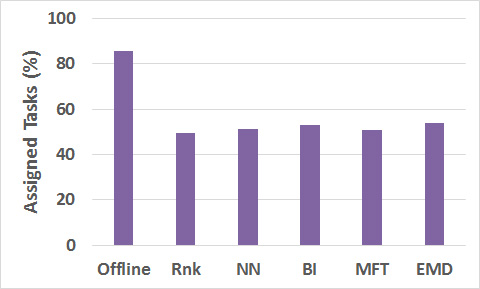
\includegraphics[width = 0.6\columnwidth]{figures/off_vs_on.jpg}
	\vspace{-0.1in}
	\caption{Online Vs. Offline}\label{fig:off_vs_on}
\end{figure}

The experimental results in \cref{fig:off_vs_on} show that the online algorithms perform within \%55-65 of the optimal solution. These experimental results are consistent with studies that indicate in the online assignment problem with random inputs, greedy algorithms achieve a competitive ratio of $1 - \frac{1}{e}$ \textcolor{red}{\textbf{provide ref}}.

\subsection{Scalability}
We measure the scalability of the proposed framework in \cref{sec:onlinealgo} on various aspects. First we show that the size of the workload is irrelevant in the performance of the online algorithms. Following that we show the affect of task/worker arrival rate in our framework.

The first set of experiments in this part focus on the size of the workload; i.e., the total number of tasks. Increasing the workload size, will only increase the duration of the simulation.

\begin{table}[h]
\begin{center}
\begin{tabular}{| l || c | c | c | c | c |} \hline
Workload Size	&	Rnk		&	NN		&	BI		&	MFT		&	EMD		\\ \hline
1K				&	70.44	&	74.64	&	74.6	&	74.56	&	76.52	\\ \hline
10K				&	70.62	&	74.12	&	74.02	&	76.32	&	78.78	\\ \hline
100K			& 	69.95	&	73.13	&	73.13	&	76.55	&	78.52	\\ \hline
1M				&	70.22	&	74.41	&	74.58	&	77.18	&	79.12	\\ \hline
\end{tabular}
\vspace{-0.1in}
\caption{\small{\% of assigned tasks for different workload sizes}}
\label{tab:size_perc}
\end{center}
\end{table}
\vspace{-0.3in}
\begin{table}[h]
\begin{center}
\begin{tabular}{| l || c | c | c | c | c |} \hline
Workload Size	&	Rnk		&	NN		&	BI		&	MFT		&	EMD		\\ \hline
1K				&	0.38	&	0.34	&	0.42	&	0.49	&	12.28	\\ \hline
10K				&	0.40	&	0.34	&	0.43	&	0.41	&	10.72	\\ \hline
100K			& 	0.46	&	0.34	&	0.43	&	0.53	&	12.47	\\ \hline
1M				&	0.45	&	0.35	&	0.44	&	0.51	&	12.92	\\ \hline
\end{tabular}
\vspace{-0.1in}
\caption{\small{average time (ms) required to assign a single task}}
\label{tab:size_time}
\end{center}
\end{table}
\vspace{-0.3in}
\begin{table}[h]
\begin{center}
\begin{tabular}{| l || c | c | c | c | c |} \hline
Workload Size	&	Rnk		&	NN		&	BI		&	MFT		&	EMD		\\ \hline
1K				&	51.58	&	35.75	&	35.50	&	50.09	&	53.94	\\ \hline
10K				&	53.80	&	35.13	&	35.00	&	51.80	&	54.98	\\ \hline
100K			& 	53.03	&	35.17	&	34.94	&	51.10	&	54.37	\\ \hline
1M				&	54.39	&	35.58	&	35.38	&	51.27	&	55.79	\\ \hline
\end{tabular}
\vspace{-0.1in}
\caption{\small{average traveled distance (mile) per completed task}}
\label{tab:size_dist}
\end{center}
\end{table}

\cref{tab:size_perc,tab:size_time,tab:size_dist} show the percentage of assigned tasks, average run-time to assign a task and average traveled distance per completed task do not change significantly even if the workload size is increased by orders of magnitude.

In practice, our proposed framework for the online algorithms acts similar to a \emph{complex event processing (CEP)} engine \cite{Luckham01}. We can measure the scalability of such systems by their throughput; the number of tasks processed per second. 